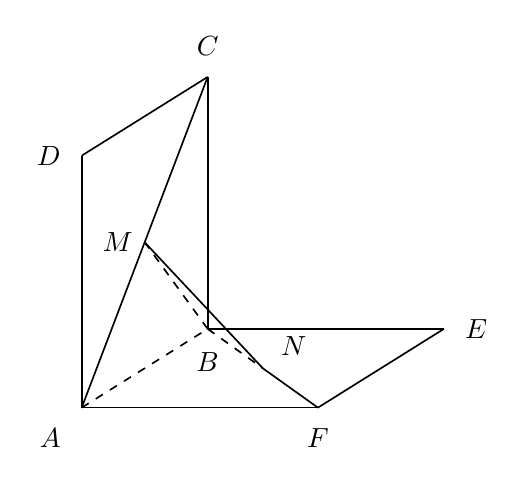
\begin{tikzpicture}[line width=.6pt, font=\normalsize]
\coordinate (A) at (0,0);
\coordinate (B) at (1.6,1.0);
\coordinate (C) at (1.6,4.2);
\coordinate (D) at (0.0000000000,3.2000000000);
\coordinate (M) at (0.8000000000,2.1000000000);
\coordinate (F) at (3.0,0);
\coordinate (N) at (2.3000000000,0.5000000000);
\coordinate (E) at (4.6000000000,1.0000000000);
% left square ABCD outline (AB hidden)
\draw (A) -- (D);
\draw (D) -- (C);
\draw (C) -- (B);
\draw (C) -- (M) -- (A);
\draw[dashed] (A) -- (B);
% right square ABEF outline (AB hidden)
\draw (A) -- (F);
\draw (F) -- (E);
\draw (E) -- (B);
% diagonal BF of second square, N on BF
\draw[dashed] (B) -- (N);
\draw (N) -- (F);
% interior segments
\draw[dashed] (B) -- (M);
\draw (M) -- (N);
% labels with clearance
\node[below left=4pt] at (A) {$A$};
\node[below=5pt] at (B) {$B$};
\node[above=4pt] at (C) {$C$};
\node[left=4pt] at (D) {$D$};
\node[left=3pt,inner sep=1pt] at (M) {$M$};
\node[right=4pt] at (E) {$E$};
\node[below=4pt] at (F) {$F$};
\node[above right=4pt,xshift=-1pt,yshift=-3pt] at (N) {$N$};
\end{tikzpicture}
